(a) From HW~\ref{hw:vtol}.\ref{chap:transfer_function_models}, the transfer function for the VTOL altitude loop is 
\begin{equation}\label{eq:hw_vtol_bode_altitude_tf}
P_{in}(s) = \frac{0.667}{s^2}.
\end{equation}
In Bode canonical form we have
\[
P_{in}(j\omega) = \frac{0.667}{(j\omega)^2}
\]
Therefore
\[ 
20\log_{10}\abs{P_{in}(j\omega)}=
	20\log_{10} 0.667 
	-40\log_{10}\abs{\omega}.
\]
Therefore, the Bode plot for magnitude will be the graphical addition of a constant gain, and a line with slope of -40~dB/decade.
Similarly, the phase is given by
\[
\angle P_{in}(j\omega) = 
	\angle 0.667 
	- \angle (j\omega)
	- \angle (j\omega) = 0 - 90 - 90 = -180~\text{degrees}.
\]
The straight line approximation as well as the Bode plot generated by Matlab are shown in Figure~\ref{fig:hw_vtol_altitude_bode}.
\begin{figure}[H]
   \centering
   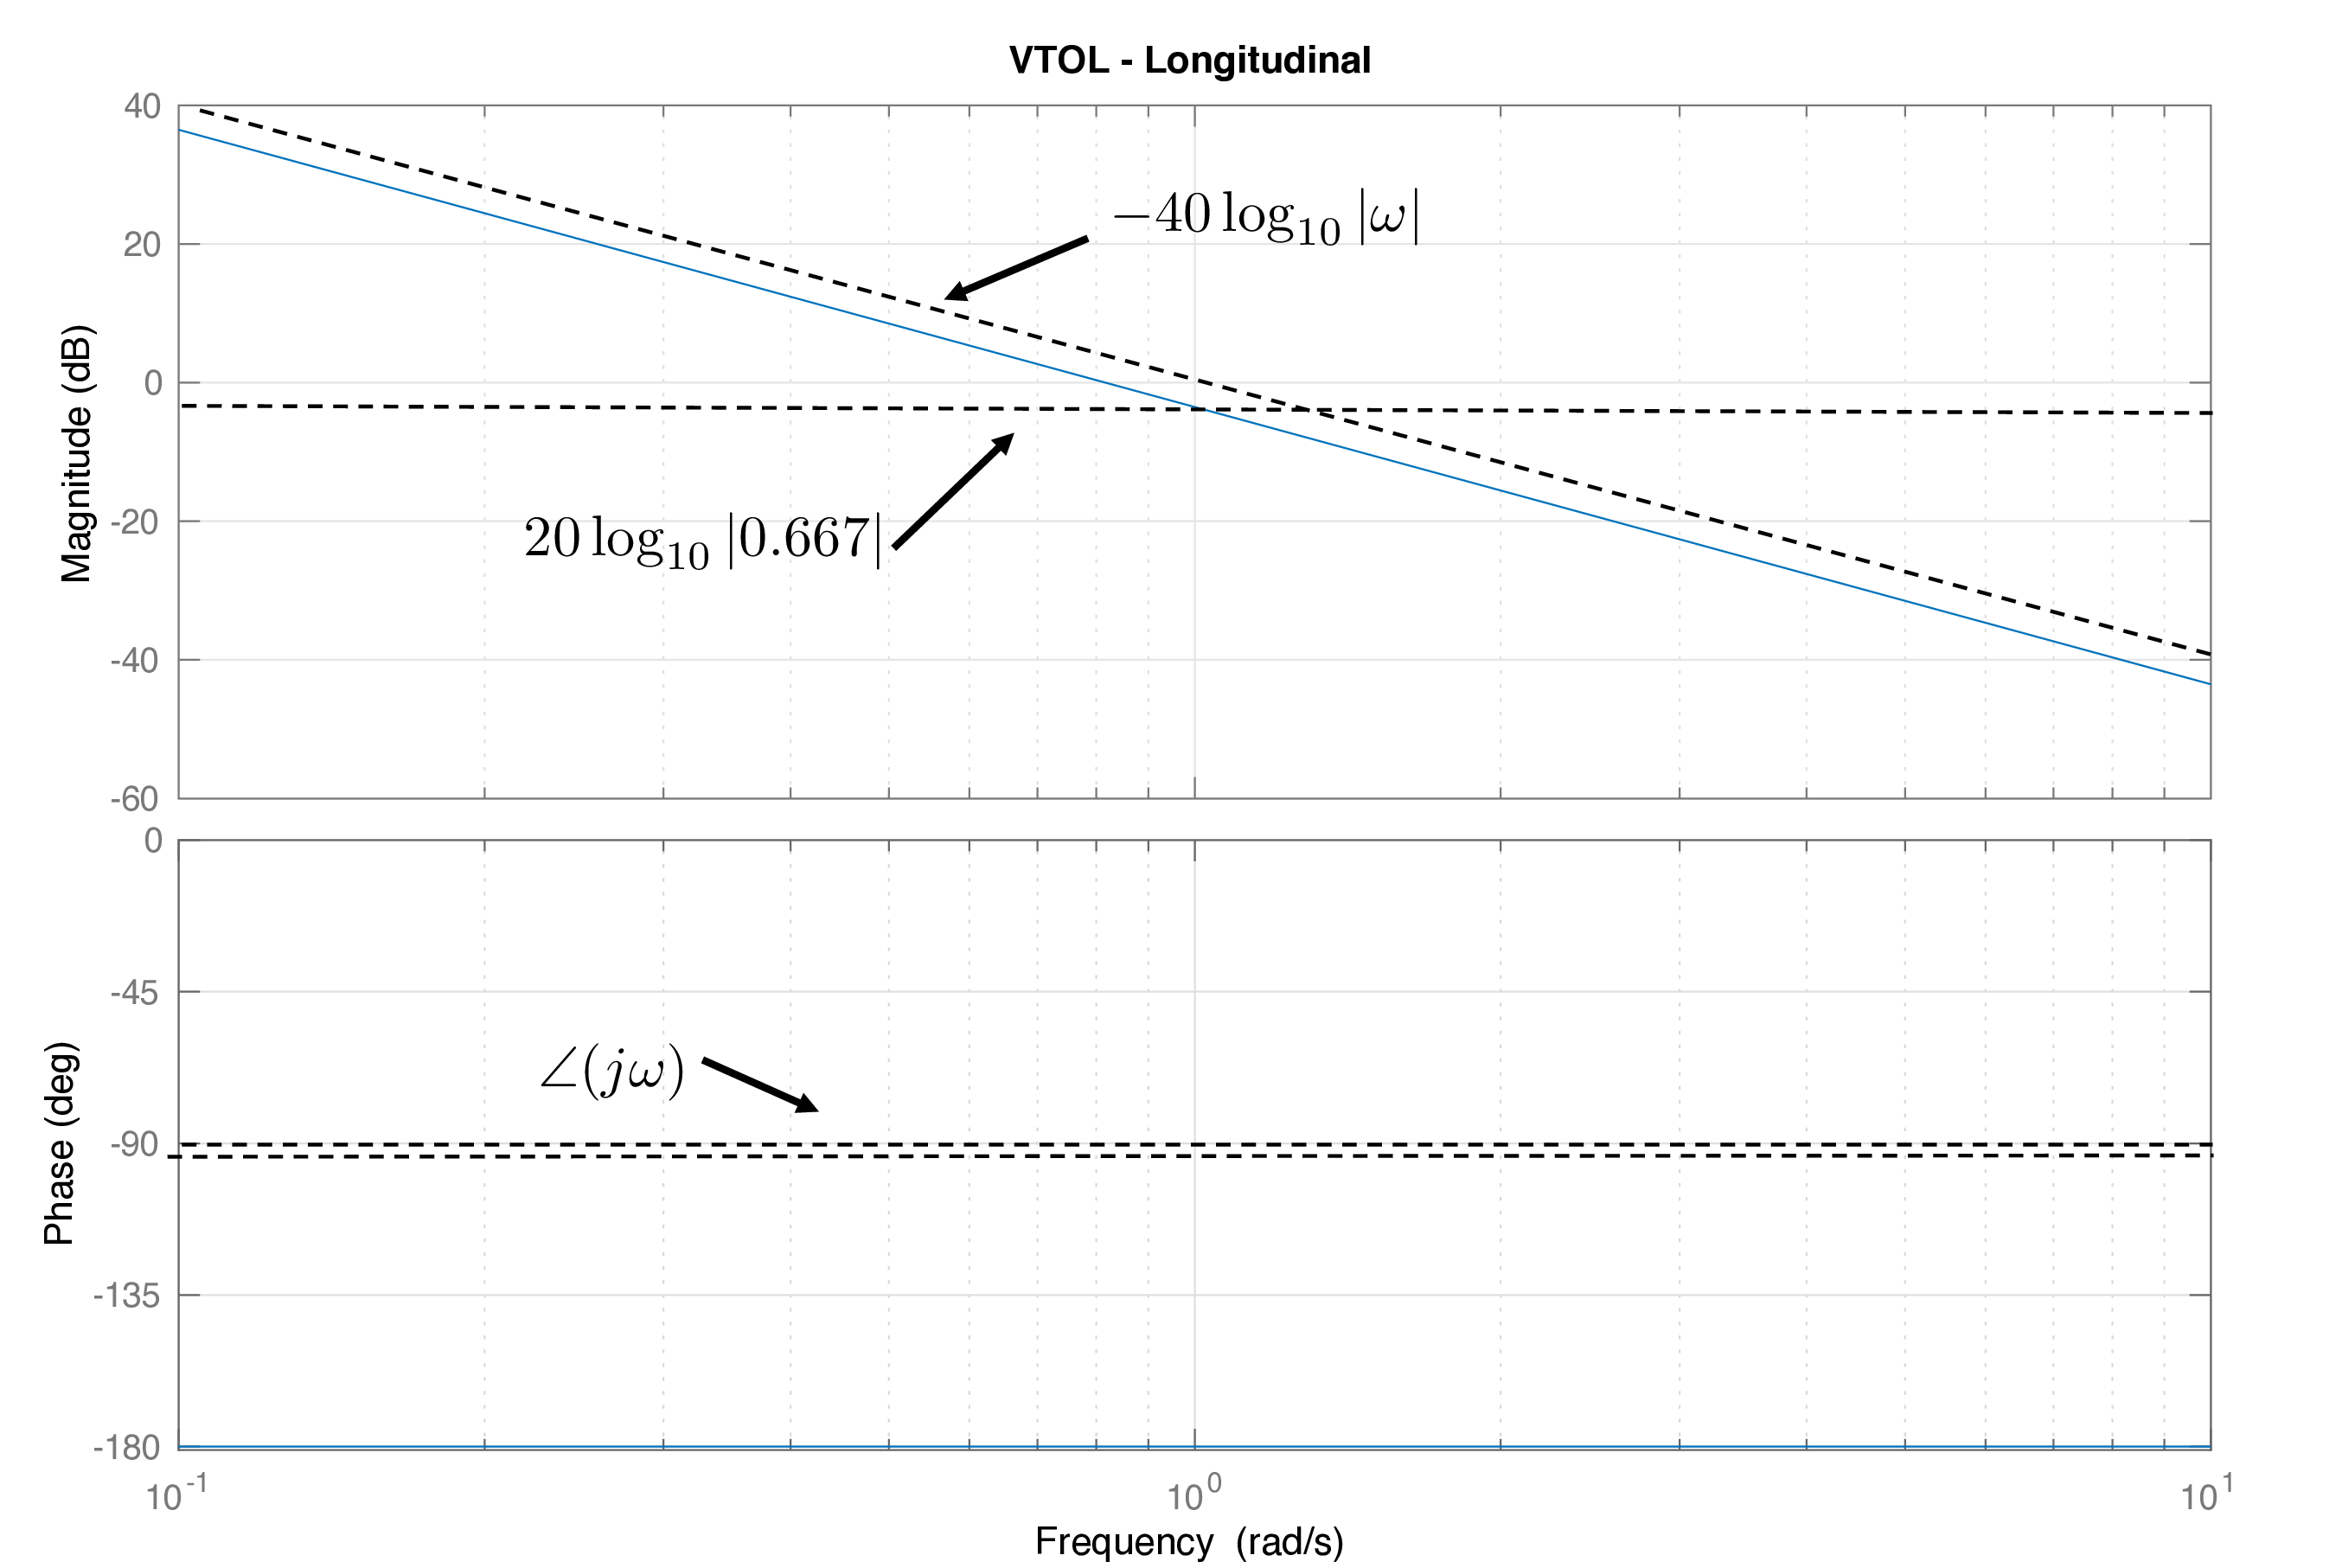
\includegraphics[width=0.9\textwidth]{6_design_studies/figures/hw_vtol_altitude_bode.pdf}
   \caption{Bode plot for the transfer function given in Equation~\eqref{eq:hw_vtol_bode_altitude_tf}.}
   \label{fig:hw_vtol_altitude_bode}
\end{figure}
%The Matlab command to generate the Bode plot is
%\begin{lstlisting}
%>> P = tf([0.667], [1, 0, 0]);
%>> figure(1), clf, bode(Pin), grid on
%\end{lstlisting}
The Python command to generate the Bode plot is
\begin{lstlisting}
	>> import matplotlib.pyplot as plt
	>> import control as cnt
	>> P = tf([0.667], [1, 0, 0]);
	>> plt.figure(1), clf, cnt.bode_plot(P), grid on
\end{lstlisting}

(b) From HW~\ref{hw:vtol}.\ref{chap:transfer_function_models}, the transfer function for the inner loop of the VTOL lateral system is 
\begin{equation}\label{eq:hw_vtol_lateral_bode_in_tf}
P_{in}(s) = \frac{20.33}{s^2}.
\end{equation}
In Bode canonical form we have
\[
P_{in}(j\omega) = \frac{20.33}{(j\omega)^2}
\]
Therefore
\[
20\log_{10}\abs{P_{in}(j\omega)}=
	20\log_{10} 20.33 
	-40\log_{10}\abs{\omega}.
\]
Therefore, the Bode plot for magnitude will be the graphical addition of a constant gain, and a line with slope of -40~dB/decade.
Similarly, the phase is given by
\[
\angle P_{in}(j\omega) = 
	\angle 20.33 
	- \angle (j\omega)
	- \angle (j\omega) = 0 - 90 - 90 = -180~\text{degrees}.
\]
The straight line approximation as well as the Bode plot generated by Matlab are shown in Figure~\ref{fig:hw_vtol_lateral_bode_in}.
\begin{figure}[H]
   \centering
   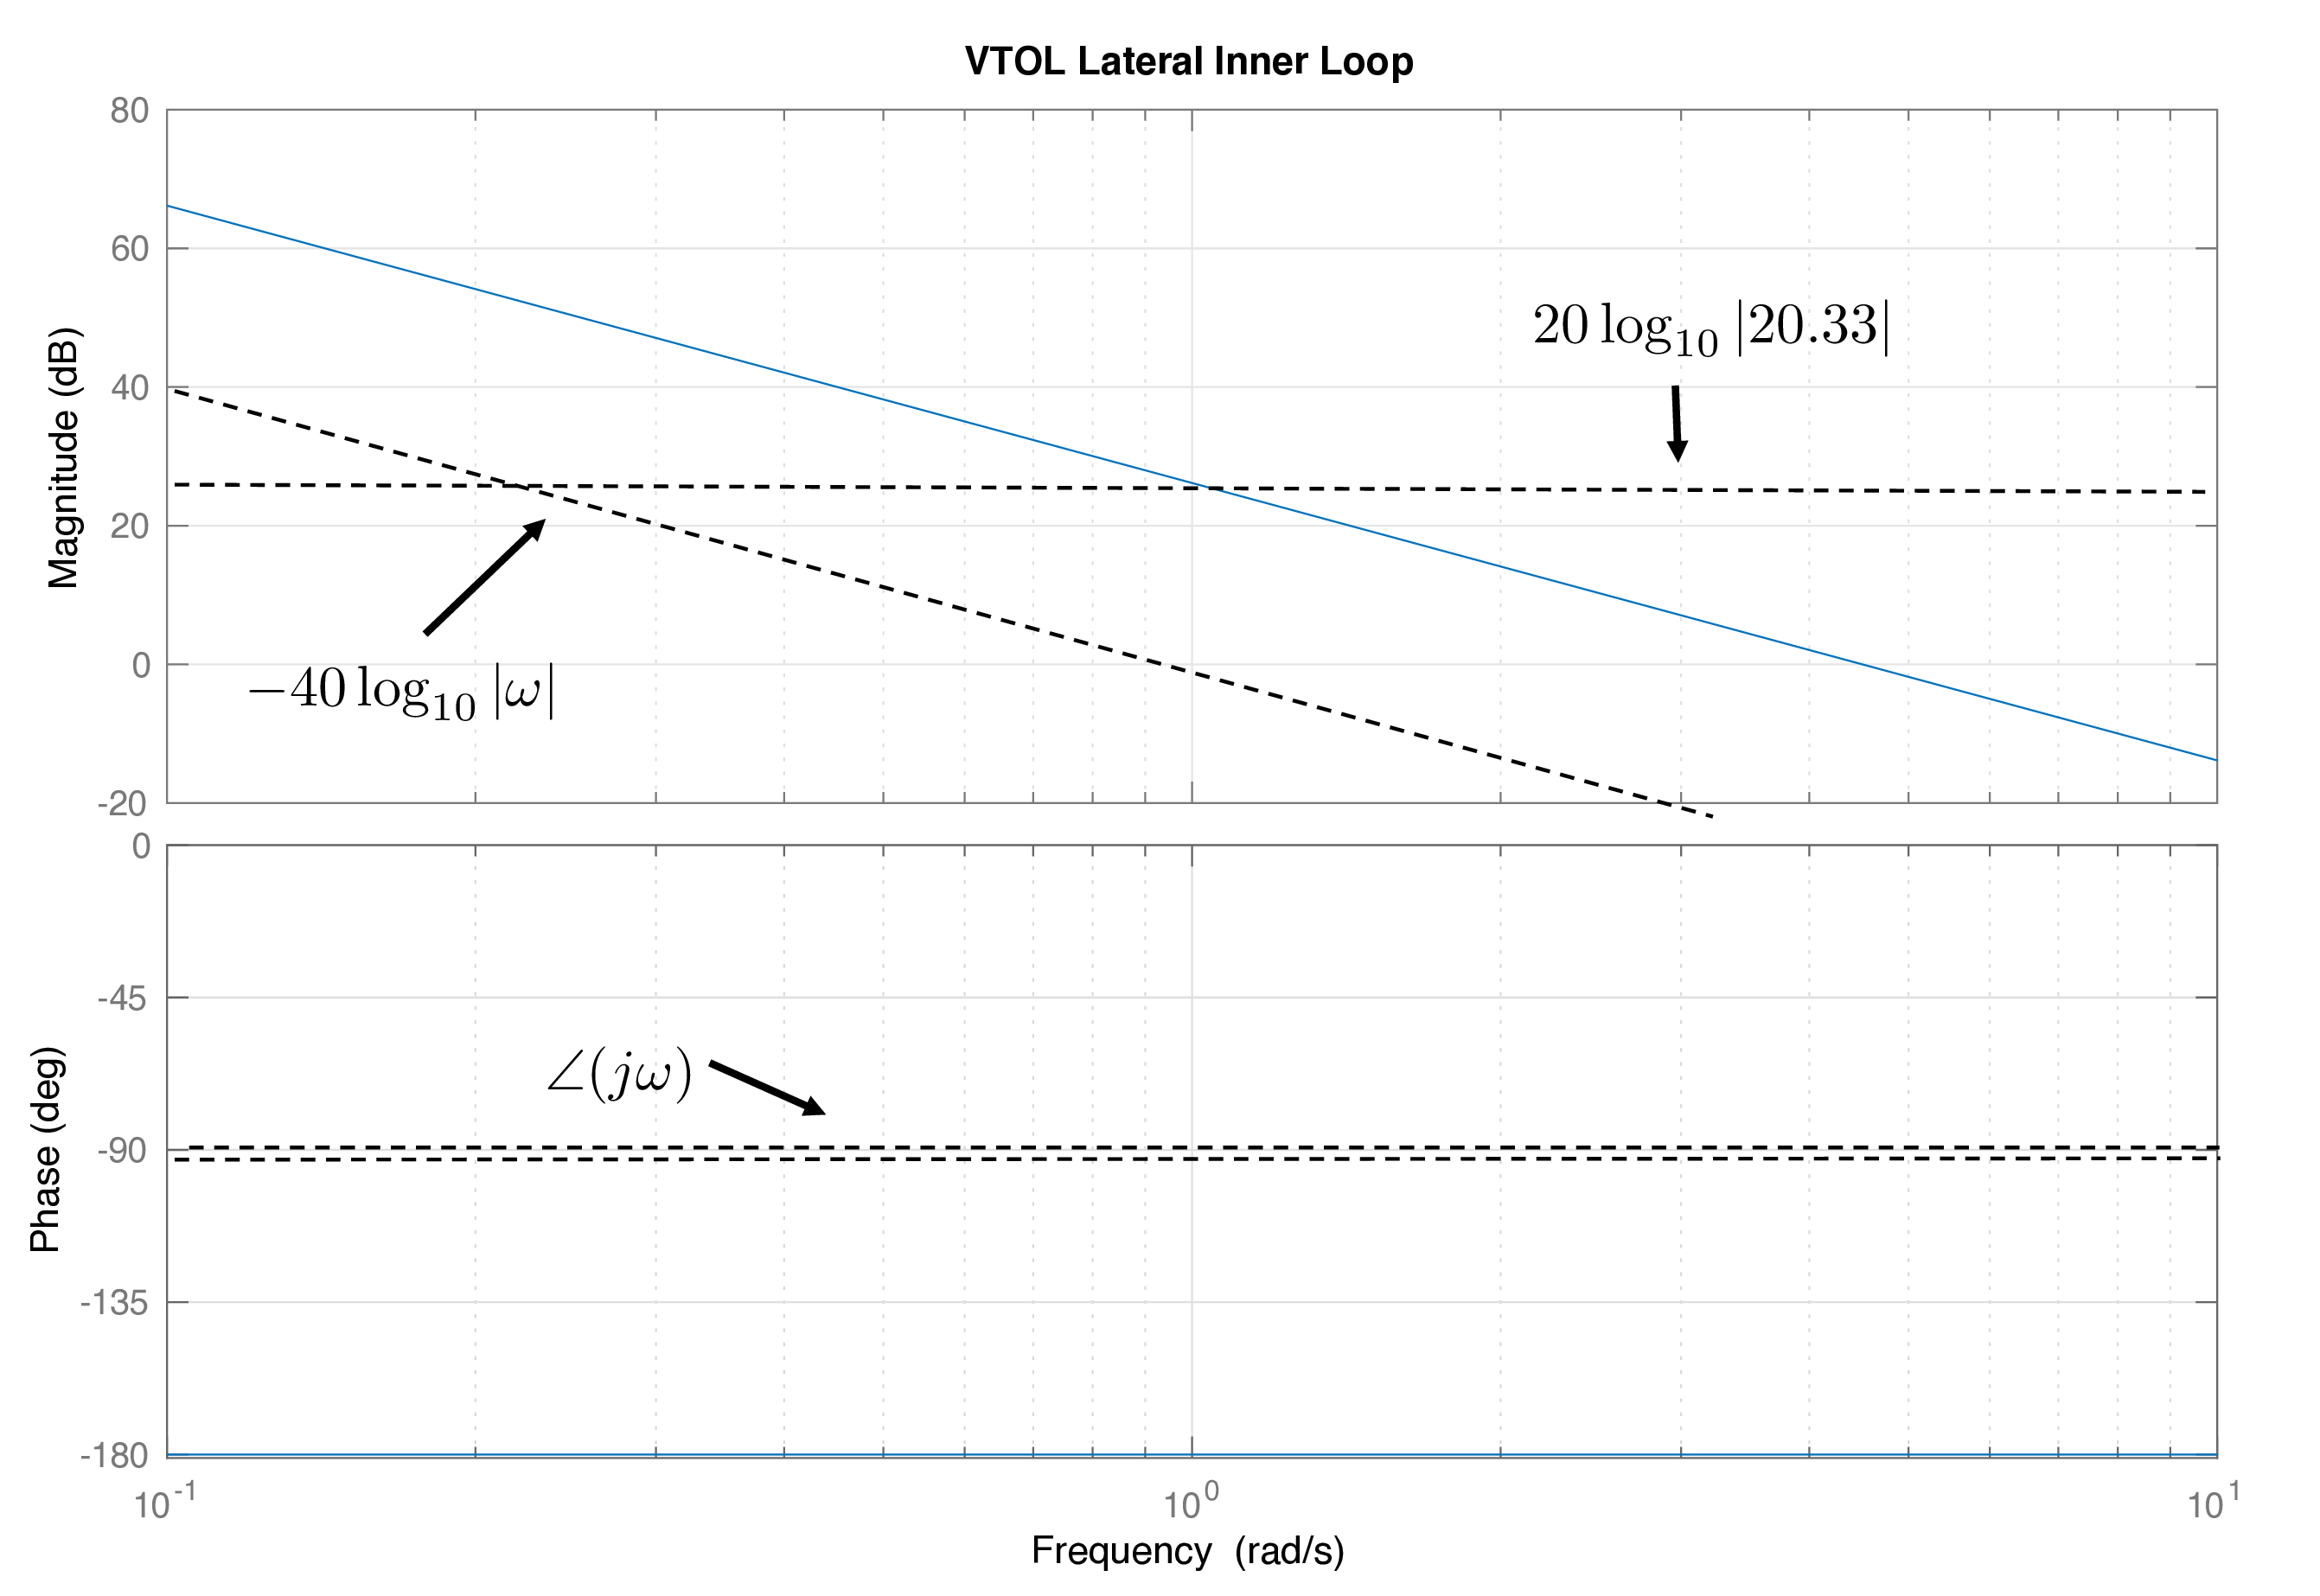
\includegraphics[width=0.9\textwidth]{6_design_studies/figures/hw_vtol_lateral_bode_in.pdf}
   \caption{Bode plot for the transfer function given in Equation~\eqref{eq:hw_vtol_lateral_bode_in_tf}.}
   \label{fig:hw_vtol_lateral_bode_in}
\end{figure}
%The Matlab command to generate the Bode plot is
%\begin{lstlisting}
%>> Pin = tf([20.33], [1, 0, 0]);
%>> figure(1), clf, bode(Pin), grid on
%\end{lstlisting}
The Python command to generate the Bode plot is
\begin{lstlisting}
	>> import matplotlib.pyplot as plt
	>> import control as cnt
	>> Pin = tf([20.33], [1, 0, 0]);
	>> plt.figure(1), clf, cnt.bode_plot(Pin), grid on
\end{lstlisting}

(c) From HW~\ref{hw:vtol}.\ref{chap:transfer_function_models}, the transfer function for the VTOL lateral system is 
\begin{equation}\label{eq:hw_vtol_lateral_bode_tf_out}
P(s) = \frac{-a}{s(s+b)} = \frac{-9.81}{s(s+0.0667)},
\end{equation}
where
\begin{align*}
a &= -\frac{F_e}{m_e+2m_r} \\
b &= \frac{\mu}{m_c+2m_r}.	
\end{align*}
In Bode canonical form we have
\[
P(j\omega) = \frac{-147.1}{(j\omega)(1+j\frac{\omega}{0.0667})}
\]

Therefore
\[
20\log_{10}\abs{P(j\omega)}=
	20\log_{10} 147.1 
	-20\log_{10}\abs{j\omega}
	-20\log_{10}\abs{1+j\frac{\omega}{0.0667}}.
\]
Therefore, the Bode plot for magnitude will be the graphical addition of a constant gain, an integrator, and a pole.
Similarly, the phase is given by
\[
\angle P(j\omega) = 
	\angle -147.1
	- \angle (j\omega)
	- \angle (1+j\frac{\omega}{0.1}).
\]
The straight line approximation as well as the Bode plot generated by Matlab are shown in Figure~\ref{fig:hw_vtol_lateral_bode_out}.
\begin{figure}[H]
   \centering
   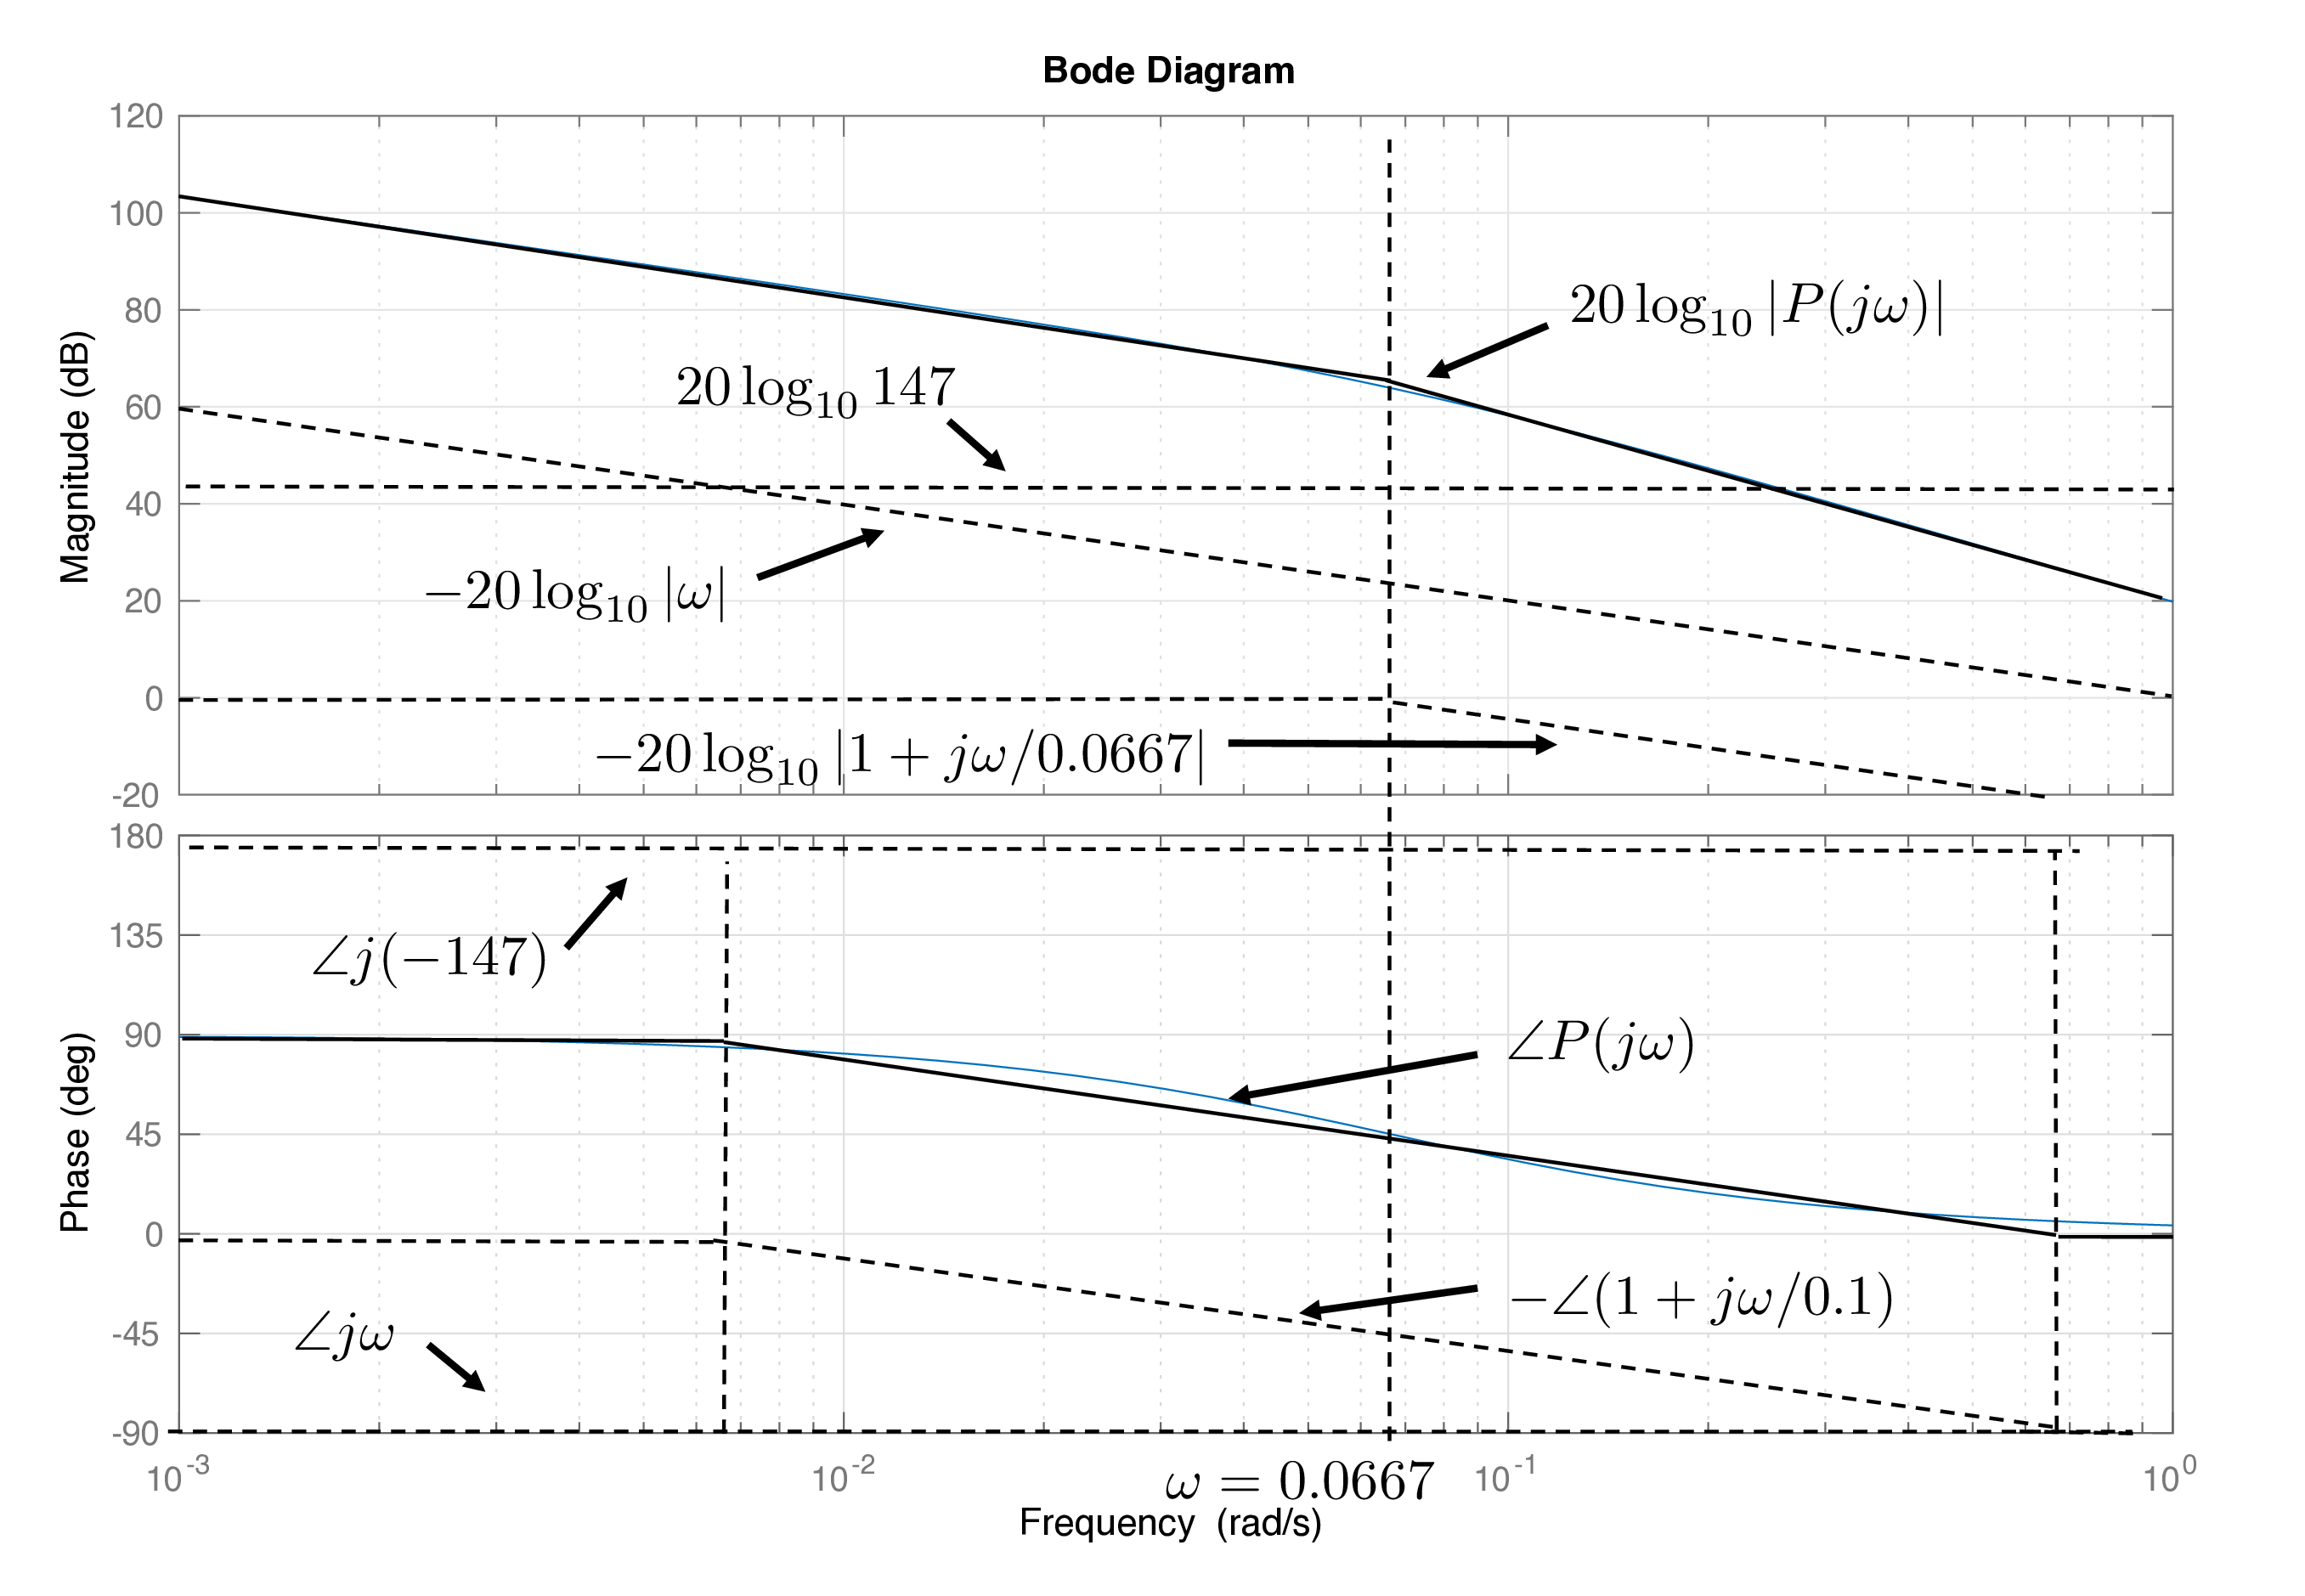
\includegraphics[width=0.9\textwidth]{6_design_studies/figures/hw_vtol_lateral_bode_out.pdf}
   \caption{Bode plot for the transfer function given in Equation~\eqref{eq:hw_vtol_lateral_bode_tf_out}.}
   \label{fig:hw_vtol_lateral_bode_out}
\end{figure}

%The Matlab command to generate the Bode plot is
%\begin{lstlisting}
%>> Pout = tf([-9.8],[1, 0.0667, 0]);
%>> figure(1), clf, bode(P), grid on
%\end{lstlisting}
The Python command to generate the Bode plot is
\begin{lstlisting}
	>> import matplotlib.pyplot as plt
	>> import control as cnt
	>> Pout = tf([-9.8],[1, 0.0667, 0]);
	>> plt.figure(1), clf, cnt.bode_plot(Pout), grid on
\end{lstlisting}

